\documentclass[11pt,a4paper]{article}

\usepackage{mynotes}

\graphicspath{ {img/} }  % Define image path

\usepackage{enumitem}
\setitemize{itemsep=0.5pt}

\renewcommand{\lstlistingname}{Code}

\newcommand\menu[1]{\texttt{\color{blue}#1}}
\newcommand\file[1]{\texttt{\underline{#1}}}

\addbibresource{hemi_photo_guide.bib}

\title{Hemispherical photography for the estimation of forest canopy traits}
\date{\today}
\author{John L. Godlee}

\begin{document}

\maketitle

\tableofcontents
\newpage

\section{Introduction}

This guide serves as an introduction to the use of hemispherical photography for estimating forest tree canopy traits in ecological research. Much of this guide has been informed by personal fieldwork, along with scattered references found throughout the scientific and practitioner literature. This guide is an attempt to bring those ideas into a cohesive resource which assumes little prior knowledge of the technique. This guide focuses on practical application of hemispherical photography, rather than being an in-depth analysis of the science of optics. It is designed to provide novice users with the means to obtain robust results quickly for use in their research. The manual contains a number of checklists for fieldwork which the user is encouraged to adapt for their own purposes and take into the field to serve as a reminder of best practice. Analysis of hemispherical photographs is covered with an effort to stick to free, open-source, and actively maintained software in order to maximise accessibility, and to ensure that the guide remains relevant into the future.

\section{What is hemispherical photography?}

Hemispherical photography is a technique where plant canopy traits are estimated from photographs taken using an extreme wide-angle or fisheye camera lens. Hemispherical photography is most commonly used to estimate the canopy cover of trees in a forest setting \citep{Seidel2011, Macfarlane2014}, and this is the focus of the current guide. 
\section{Measurements of forest tree canopies}

Hemispherical photographs can be analysed in multiple ways to provide different metrics related to the form of the forest canopy. All these metrics are related and rely fundamentally on the classification of pixels in the photo into either plant material or sky. Different metrics are used depending on the convention of the chosen field of research and according to the research question being asked. Some common metrics are:

\begin{itemize}
	\item{Gap fraction - Proportional coverage of plant canopy material as viewed from a single point with some given angular field of view (\%), AKA site factor or canopy closure \citep{Anderson1964}.}
	\item{Canopy cover - Proportional coverage of plant canopy material per unit ground area covered (\%).}
	\item{Leaf/Plant Area Index (LAI/PAI) - Area of leaf (LAI) or plant (PAI) per unit ground area (m\textsuperscript{2} m\textsuperscript{-2}).}
\end{itemize}

\begin{figure}[H]
\centering
	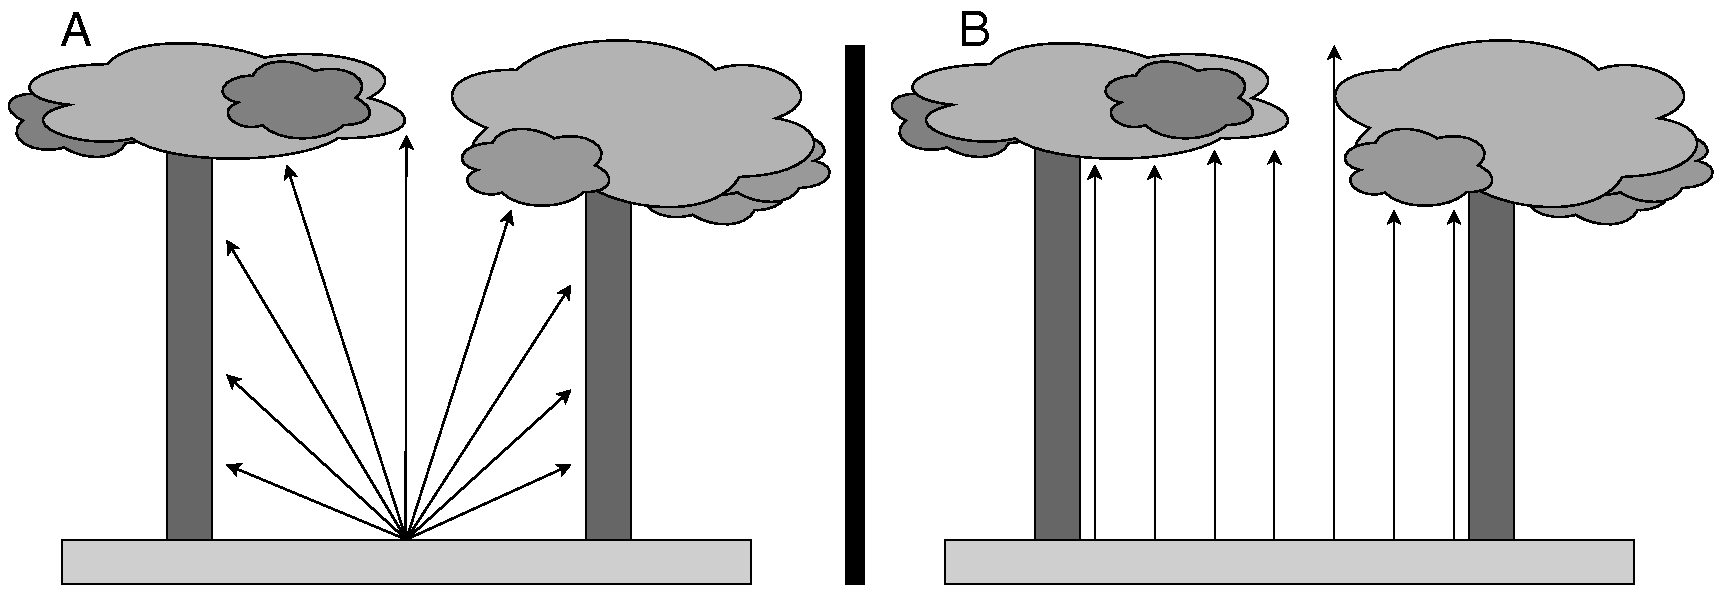
\includegraphics[width=\textwidth]{closure.drawio.pdf}
	\caption{Gap fraction (left) measured as the sky obscured by trees as measured from a single point, compared with canopy cover (right) measured as the vertical projection of tree material onto the ground (Adapted from \citealt{Jennings1999}).}
	\label{closure}
\end{figure}

\section{Hemispherical photos in the field}

\subsection{Capturing informative photos}

Taking hemispherical photos under field conditions which are representative of the forest canopy requires the careful balancing of camera settings. Images must be properly exposed and without visual aberrations which would otherwise bias analysis. Confident use of the many settings available on a modern DSLR camera is necessary to adjust for environmental conditions which may change throughout the day to gather consistent and informative images.

Some common issues which create bias in results:

\begin{itemize}
	\item{Lens flare - Bright sunlight reflects within the lens mechanism due to material imperfections in the lens glass, causing haze and starburst artefacts in the image (\autoref{lens_flare}).}
	\item{Blooming - An over-saturated part of the image bleeds over into other pixels on the image sensor during image capture. This is the most common problem in hemispherical photography.}
	\item{Obstructions between camera and tree canopy - Understorey vegetation, man-made objects, people etc. can all contribute to an inaccurate estimate of the area of plant material in the frame.}
\end{itemize}

\begin{figure}[H]
\centering
	\includegraphics[width=0.6\textwidth]{lens_flare}
	\caption{An example of a hemispherical photo with excessive lens flare. In this example, the canopy gap fraction will be over-represented as the bright lens flare will be classified as sky during the binarization process. This photo should be discarded from further analysis.}
	\label{lens_flare}
\end{figure}

There is no standard protocol for hemispherical photography, capturing an informative image relies on manual adjustment of three key camera settings to balance the image exposure and sharpness:

\begin{itemize}
	\item{Shutter speed - the length of time the shutter is open while the
		image is being captured}
	\item{Lens aperture - the size of the hole through which light enters into
		the camera lens}
	\item{ISO - analogous to the sensitivity of the sensor to incoming light}
\end{itemize}

Below is a checklist to guide you in taking informative hemispherical photographs: 

\begin{itemize}
	\item{Take photos under a uniformly overcast sky where possible, ideally before the sun has risen high in the sky, or just before sunset. This avoids lens flare and increases contrast between plant and sky. In the morning the photos are generally better due to the quality of the light and the generally more consistent cloud cover. At high latitudes you will have a longer suitable period to capture photos than in the tropics.}
	\item{Ensure that the camera is level on the tripod and the lens is pointing straight up. Use a spirit level attached to the camera hotshoe to do this.}
	\item{Adjust the tripod so that the top of the camera lens is 1 m above the ground, or above any understorey vegetation you wish to exclude from the analysis, whichever is higher.} 
	\item{Turn the camera so the top of the camera body is facing north, bring a compass! This ensures that the top of the captured photo is also facing north, which is necessary for calculating LAI.}
	\item{Make use of the camera's visual display, if there is one, to get a good view of the photo before you take it.}
	\item{Set the camera. Note that these settings assume you are using the
		``ideal list of products'' found later in this guide:}
		\begin{itemize}
			\item{Manual shooting mode}
			\item{Manual focus}
			\item{Set the focus to infinity}
			\item{Set the exposure compensation to -0.7. This makes thresholding the image easier later on, see \citet{Zhang2005}}
			\item{Capture fine \file{.jpg} and RAW images at the same time}
			\item{Ensure the camera time and date is accurate (this is purely for ease of matching photos to sites during analysis)}
			\item{Set the Aperture to about 7. This is only a guideline.}
			\item{Adjust the ISO and shutter speed so the photo is neutrally exposed but the shutter speed is always over 1/60sec, otherwise you will introduce camera shake when you capture the photo. If it's windy check the photos for blurry tree branches and adjust the shutter speed accordingly.}
			\item{If the camera attempts to intelligently rotate photos based on the camera orientation, disable this feature and make sure all photos are captured in landscape orientation, never portrait.}
		\end{itemize}
	\item{Make sure everybody ducks down below the camera when the image is taken!}
	\item{Cover the lens with the lens cap between photos to prevent accidents.}
\end{itemize}

A daily kit list for taking hemispherical photos:

\begin{itemize}
	\item{Camera with appropriate fisheye lens}
	\item{Lens cap}
	\item{Lens cleaning solution and lens cloth}
	\item{Tripod}
	\item{At least 2 fully charged batteries for camera}
	\item{2 SD cards}
	\item{Spirit level hotshoe attachment for camera}
	\item{Compass}
	\item{Notebook and pencil}
	\item{GPS unit}
	\item{Tape measure > 2 m}
	\item{Waterproof bag to cover camera}
\end{itemize}

An ideal list of products for a high quality DSLR camera setup:

\begin{itemize}
	\item{Nikon D750 DSLR Camera Body}
	\item{Sigma 8 mm f3.5 Circular Fisheye EX DG For Nikon Lens}
	\item{Hotshoe Fit Spirit Level}
	\item{Integral USB SD Card Reader}
	\item{2x Sandisk Ultra 30 MB/s SDHC Card 16 GB Class 10}
	\item{Hard peli-case to fit equipment in, e.g. Peli-1520 with foam}
	\item{A sturdy tripod}
\end{itemize}

Note that the tripod needs to be able to tilt the camera so the lens points straight up. This is difficult with many tripods. Alternatively you could add a gimbal which attaches to the top of the tripod. Adding a gimbal may often work out cheaper than buying a new tripod.

\subsection{Sampling strategy}

In order to estimate the mean value of various forest canopy traits over an area of forest, multiple photos must be taken. Determining the spatial distribution of these multiple photos is therefore necessary to ensure that a representative sample of the forest canopy is achieved. The shape of the sampling area will somewhat determine the spatial pattern of photos, circular plots may require a different layout to rectangular plots and linear transects, for example.

During analysis it is common to restrict the field of view of the hemispherical photo to 60\textdegree{}. See \autoref{fov} for more information. With this in mind, a simple calculation with some sensible assumptions can estimate the minimum distance of photos to avoid pseudo-replication of the canopy area:

\begin{equation}
	D = 2D_{\theta} = 2(h \tan{\theta})
\end{equation}

where $\theta$ is the angular field of view in degrees, $h$ is the height from the camera lens to the base of the canopy, and $D$ is the minimum distance of photos to avoid pseudo-replication of canopy area.

\begin{figure}[H]
\centering
	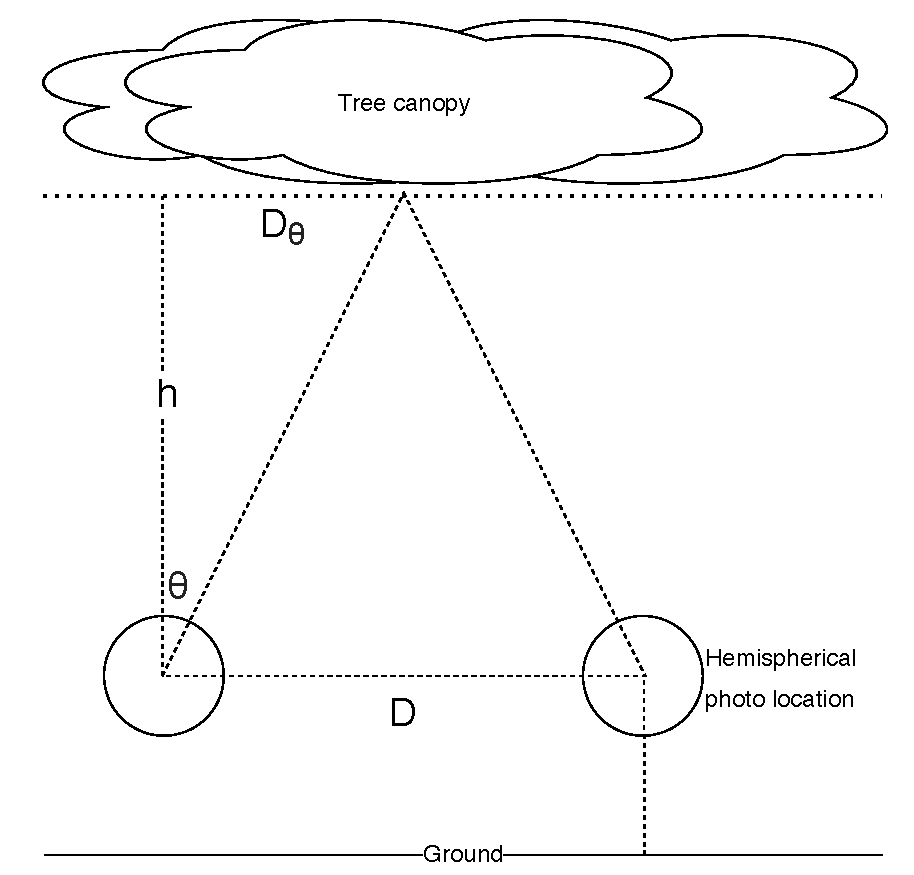
\includegraphics[width=0.5\textwidth]{canopy_trig.drawio}
	\caption{Schematic diagram of the measurements used when calculating the minimum distance between hemispherical photo locations.}
	\label{canopy_trig}
\end{figure}

\subsection{Setting the focus to infinity} 

My assumption has always been that when taking hemispherical photos of forest canopies, the focus of the lens should be set to infinity. While this knowledge is repeated throughout the literature, it is difficult to find much discussion on \textit{why} this is the case. What follows is a series of quotes from the literature on the discussion of setting the lens focus to infinity.

\begin{minipage}{\linewidth}
\begin{framed}
We used a Nikon MF-16 camera and a Nikkor 8-mm fish-eye lens with TriX ASA 400 film, a red filter to increase sharpness of leaf edges, and the \textit{focus set to infinity}.

-- \citealt{Englund2000}
\end{framed}
\end{minipage}

\begin{minipage}{\linewidth}
\begin{framed}
The lens was set to a small aperture and \textit{focused on infinity} (Frazer et al. 2001; Zhu et al. 2003)

-- \citealt{Hu2009}
\end{framed}
\end{minipage}

\begin{minipage}{\linewidth}
\begin{framed}
Exposure settings were selected to obtain the best contrast between foliage and sky and making the last one appear white (cloudy sky offers the best condition in this context). The camera was used in automatic mode using the parameters fixed in FISHEYE1 lens mode (\textit{focus set to infinity}, widest zoom, metering center-weighted), and the shutter speed was varied automatically by the camera.

-- \citealt{Paletto2009}
\end{framed}
\end{minipage}

This next quote comes from a paper which many others reference when describing proper protocol for taking hemispherical photos: 

\begin{minipage}{\linewidth}
\begin{framed}
Unlike the Nikon F, the digital camera did not allow full manual control of both the shutter speed and lens aperture. We therefore \textit{set the autofocus, exposure mode, and f-stop of the digital camera to infinity}, aperture priority (shutter speed is set automatically by the camera), and f/2.6, respectively. 

-- \citealt{Frazer2001}
\end{framed}
\end{minipage}

While this paper is one of the most respected guides on hemispherical photography, it references an unconventional source when describing the practice of setting the focus to infinity. A downloadable tutorial series on taking high-quality digital photos, called 123di \citep{123di}. Most of this resource is behind a pay-wall, so I can't read the applicable bit. Importantly however, this paper references \textit{why} the authors set the focus to infinity, because the depth of field is practically infinite under these conditions.

\begin{minipage}{\linewidth}
\begin{framed}
Photographic images were recorded using a Sigma 8 mm f/4 fisheye lens (Sigma Corporation, Tokyo, Japan) at the highest possible resolution (3040-2008 pixels) with highest ISO setting (ISO 200). Moreover, \textit{the focus ring was set to infinity when using the fisheye lens, as depth of field is practically infinite and focusing was not required (Bockaert, 2004).}

-- \citealt{Jonckheere2005}
\end{framed}
\end{minipage}

\section{Processing hemispherical photographs}

There are many proprietary options for processing and analysing forest canopy traits from hemispherical photographs, e.g. WinScanopy, CAN-EYE. I think processing with freely available tools is more flexible, reproducible, and future-proof, and should be preferred for peer-reviewed research. This part of the guide demonstrates a workflow for processing hemispherical photos using ImageJ v1.x \citep{Schneider2012}.

\subsection{Differentiating between plant and sky}

In order to calculate various forest canopy traits it is necessary to partition the hemispherical photo into areas of plant material and sky. A straightforward method for this relies on the assumption that the sky will be much brighter than the plant material. This is largely true for a correctly exposed hemispherical photo. The checklist below describes how to partition an image based on pixel brightness, in ImageJ. This process returns an image with white pixels for sky and black pixels for plant material. Monospace blue font refers to menu items in ImageJ to be selected.

\begin{enumerate}
	\item{Open ImageJ}
	\item{\menu{File $\rightarrow$ Open}, then select an image to process.}
	\item{Visually inspect the image to see that there isn't large amounts of lens flare. See \autoref{lens_flare} for an example of lens flare. If you have lots of lens flare, the photo should be discarded.}
	\item{\menu{Image $\rightarrow$ Type $\rightarrow$ 8-bit}}
	\item{\menu{Image $\rightarrow$ Adjust $\rightarrow$ Threshold}, tick \menu{Dark background} and manually adjust the image so all sky is entirely red and the branches are grey, or as near as you can get it. Click \menu{Apply} to binarize the image.}
	\item{Save the newly thresholded image as a \file{.tif} in a separate directory. The image should have black plant material and white sky.}
	\item{Repeat for all images.}
\end{enumerate}

\begin{figure}[H]
\centering
	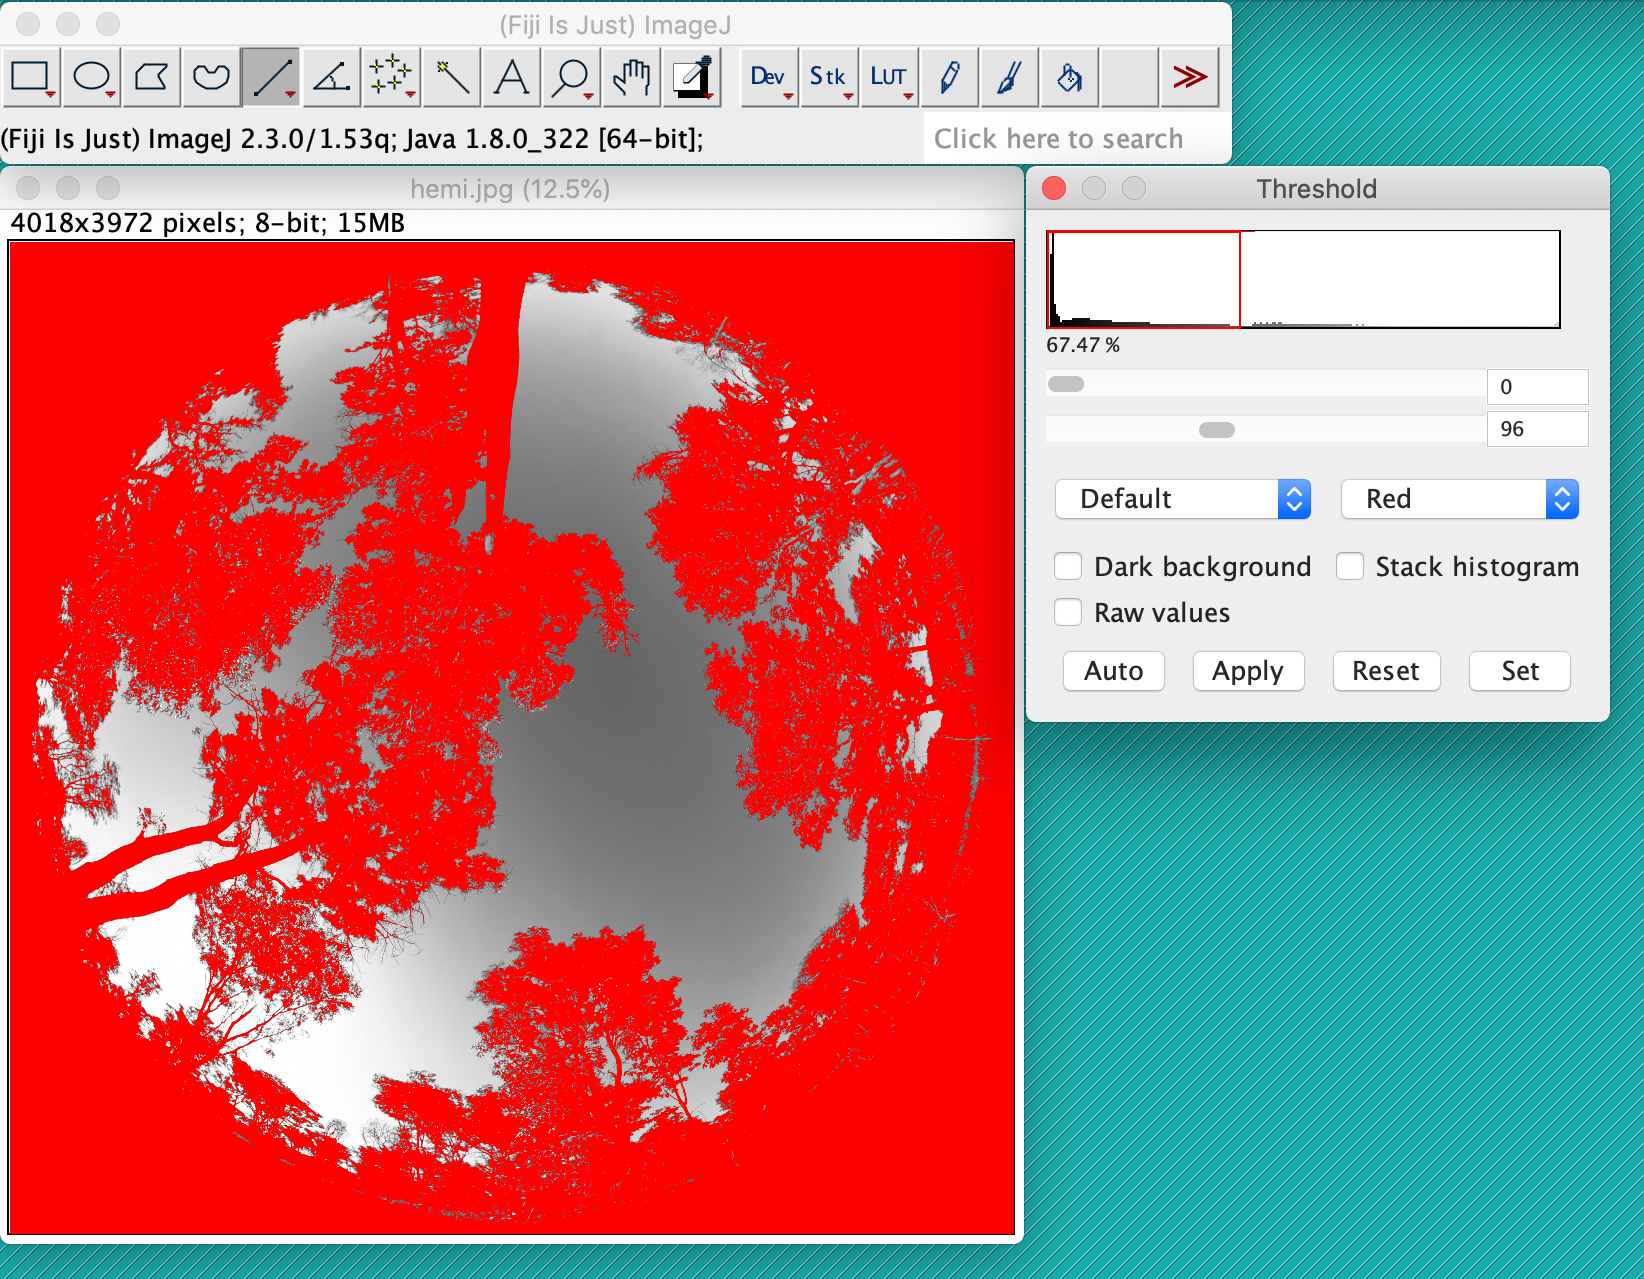
\includegraphics[width=0.8\textwidth]{threshold}
	\caption{Screenshot of the binarization thresholding process in ImageJ.}
	\label{threshold}
\end{figure}

The above process can be automated with an ImageJ macro (\autoref{binarize}), but this removes the ability to manually threshold each image, relying instead on one of a number of binarization algorithms provided in ImageJ. This technique should only be used when you are confident that all images are consistently exposed. Macros should be saved as a \file{.ijm} file and called within ImageJ with \menu{Plugins $\rightarrow$ Macros $\rightarrow$ Run..}. For a full list of macro functions available in ImageJ, consult the documentation (\url{https://imagej.nih.gov/ij/developer/macro/functions.html}). 

\begin{minipage}{\linewidth}
\lstinputlisting[label=binarize,caption=ImageJ macro to binarize all images in a nominated directory. The macro can also be found in \file{binarize.ijm} in the supplementary material.]{src/binarize.ijm}
\end{minipage}

I find that the \verb|Huang| \citep{Huang1995} binarization algorithm normally works well for thresholding canopy photos, but you should experiment with different algorithms to find the one which works best for your data. \verb|Default| is also widely appropriate for canopy photos.

An alternative to simple thresholding of 8-bit greyscale images is to use a colour thresholding technique. Plant material often reflects very little blue, while the sky generally reflects much more, so one can threshold using only the blue channel of the image (\citealt{Brusa2014}, \autoref{binarize_blue}).

\begin{minipage}{\linewidth}
\lstinputlisting[label=binarize_blue, caption=ImageJ macro to binarize images by the blue colour channel. The macro can also be found in \file{binarize\_blue\_channel.ijm}.]{src/binarize_blue.ijm}
\end{minipage}

\subsection{Cropping a circular image} \label{circle}

Sometimes, it's desirable to crop a hemispherical photo to a smaller circle with a known angle of view (zenith angle). A common convention is to crop an image to a 60\textdegree{} angular field of view. See \autoref{fov} for more information. Fisheye lenses have different projection functions which map the curved image onto a flat surface. Here is a list of common projection functions for different lenses:

\begin{itemize}
	\item{Equisolid (equal area) - $R = 2f\sin{(\theta/2)}$}
	\item{Equidistant - $R = f\theta$}
	\item{Orthographic - $R = f\sin{(\theta)}$}
	\item{Stereographic - $R = 2f\tan{(\theta/2)}$}
	\item{Thoby fisheye - $R = 1.47f\sin{(0.713\theta)}$}
\end{itemize}

\begin{figure}[H]
	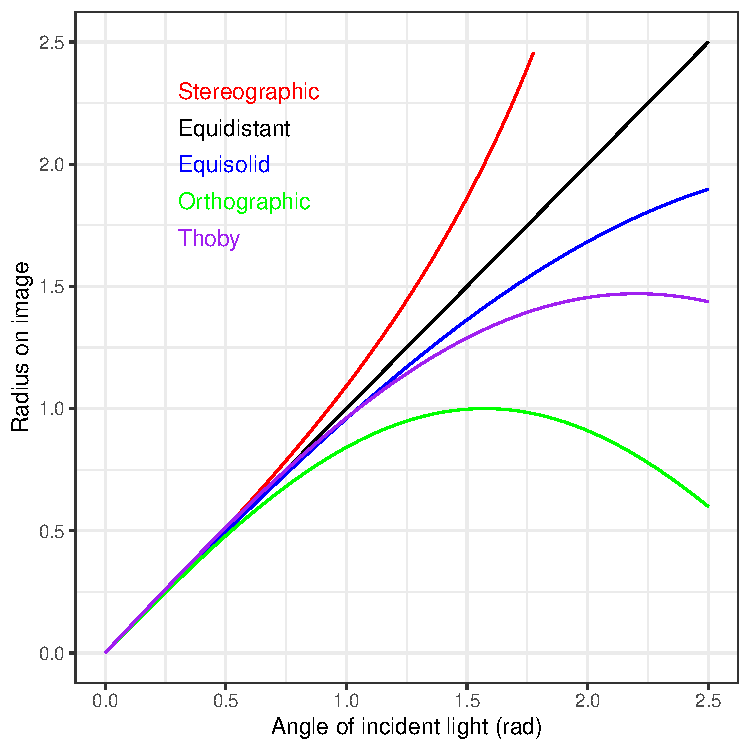
\includegraphics[width=\textwidth]{lens_proj}
	\caption{Comparison of common fisheye lens projection functions.}
	\label{lens_proj}
\end{figure}

where $R$ is the radial position of a point on the image on the sensor, $f$ is the focal length of the lens, and $\theta$ is the angle in radians of incident light on the lens. Here is a diagram of what those values equate to on the camera lens.

\begin{figure}[H]
\centering
	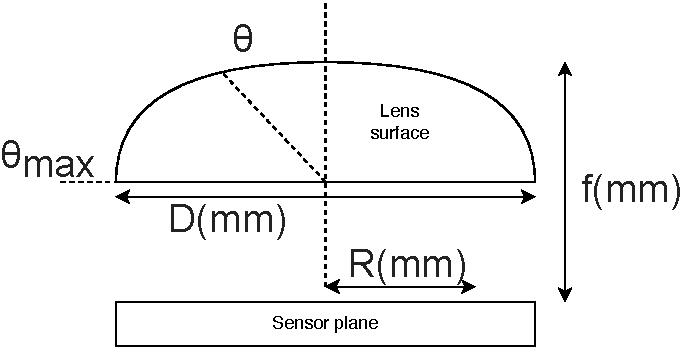
\includegraphics[width=\textwidth]{fov_diagram.drawio}
	\caption{Schematic diagram of a camera lens and sensor, demonstrating the measurements used when cropping an image to a given angular field of view.}
	\label{fov_diagram}
\end{figure}

The lens in the ``ideal product list'' (Sigma 8 mm) uses an equisolid projection. Equisolid lenses are preferred for hemispherical photography because they maintain an equal area for each pixel, i.e. a pixel projected through the lens has the same solid angle irrespective of the incident light angle. Below is a function written in the R programming language which will provide the radius of the circle in pixels for a desired angular field of view for the equisolid projection (\autoref{fov_func}).

\begin{minipage}{\linewidth}
\lstinputlisting[language=R, label=fov_func, firstline=18, lastline=32, caption=R function to calculate the pixel radius of a circle with a given zenith angle. Also found in \file{fov\_func.R} in the supplementary materials.]{src/fov_func.R}
\end{minipage}

The pixel pitch of the sensor is the real distance (in $\mu$m) from the centre of one pixel on the sensor to the centre of the next, in the case of the Sigma 8 mm it's 5.95 $\mu$m. This information can generally be found by querying the technical specifications for the camera, which may be available from the manufacturer or possibly found on online forums.

Similarly, below is a function to calculate the angular field of view of an already cropped circular image, by solving the equation for $\theta$ (\autoref{fov_theta}). 

\begin{minipage}{\linewidth}
\lstinputlisting[language=R, label=fov_theta, firstline=48, lastline=58, caption=R function to calculate the zenith angle from a cropped circular image. Also found in \file{fov\_func.R} in the supplementary materials.]{src/fov_func.R}
\end{minipage}

\subsection{Calculating gap fraction with ImageJ}

The process for calculating gap fraction is fairly simple. Basically, from the binarized \file{.tif} images you made previously, you simply count the number of pixels in the image which are sky, i.e. white in the binarized image, then divide by the total number of pixels in the image. It's slightly more complicated when the image is a circle within a larger frame, but not much.

To calculate gap fraction: 

\begin{enumerate}
	\item{Open Image}
	\item{\menu{File $\rightarrow$ Open} then select a binarized \file{.tif} image} 
	\item{\menu{Edit $\rightarrow$ Invert} to invert the colours}
	\item{\menu{Analyze $\rightarrow$ Analyze Particles..}}
		\begin{enumerate}
			\item{\menu{Size (pixel\textsuperscript{2})} = 0-infinity}
			\item{\menu{Circularity} = 0-1}
			\item{\menu{Show} = Nothing}
			\item{Check \menu{Summarize}}
		\end{enumerate}
	\item{The results should appear in a table, the gap fraction value is \menu{\%Area}}
	\item{Rinse and repeat for all images}
\end{enumerate}

\autoref{gap_frac_image} performs the same process but for a directory of images and exports a \file{.csv} spreadsheet file of the results. Remember to change the user inputs to point to where you would like images to be opened from and the spreadsheet saved to.

\begin{minipage}{\linewidth}
\lstinputlisting[label=gap_frac_image, caption=ImageJ macro to calculate the gap fraction of a full image. The macro can also be found in \file{gap\_frac\_image.ijm}.]{src/gap_frac_image.ijm}
\end{minipage}

The process is similar for a circular image such as that taken with a full frame camera and a fisheye lens, except you draw a circle selection to exclude the black uninformative parts of the image before running \menu{Analyze Particles...}. See \autoref{gap_frac_circle} for the macro. 

\begin{minipage}{\linewidth}
\lstinputlisting[label=gap_frac_circle, caption=ImageJ macro to calculate the gap fraction of a circular selection of an image. The macro can also be found in \file{gap\_frac\_circle.ijm}.]{src/gap_frac_circle.ijm}
\end{minipage}

The circular diameter of the image to fill \verb|circle_diam| can be measured in ImageJ by selecting \menu{Straight Line} from the toolbar then drawing a straight line across the centre of the circular image. Then select \menu{Analyze $\rightarrow$ Measure} to get the length of the line in the Results table. Alternatively, use the methods presented above in \autoref{circle} to crop the circular image to a particular angle of view, to exclude parts of the image closer to the ground.

\subsection{Calculating Leaf Area Index}

This part of the guide relies mostly on code written by Hans ter Steege in the HemiPhot R package \citep{Steege2018}, which ports WinPhot into the R language. Winphot was originally written by Hans ter Steege in 1997, and Hemiphot can be seen as the natural progression of this software. Winphot is now obsolete and has been unmaintained since Windows XP. The code includes functions for thresholding and binarizing images, but I prefer to do this step in ImageJ prior to analysing the images in R, because I like I have more control over how the images are thresholded this way. The snippets below describe a workflow for processing multiple binarized images in Hemiphot using R:

\vspace{0.5cm}
\begin{minipage}{\linewidth}
0. Preamble, load packages and functions.
\lstinputlisting[language=R, linerange=5-8]{src/hemiphot_example.R}
\end{minipage}

\begin{minipage}{\linewidth}
1. Read in all the previously thresholded and binarized \file{.tif} images and create an empty data frame which will later be filled with canopy trait metrics like LAI and canopy openness.
\lstinputlisting[language=R, linerange=10-21]{src/hemiphot_example.R}
\end{minipage}


\begin{minipage}{\linewidth}
	2. Set some parameters for the location the photos are being taken. Approximate location (0.1\textdegree{} latitude) is good enough for our purposes. Note that the values below are for somewhere in Africa and should be changed:
\lstinputlisting[language=R, linerange=23-27]{src/hemiphot_example.R}
\end{minipage}


\begin{minipage}{\linewidth}
3. Set some parameters for the images, cropping them to a circle and setting the threshold. Even if the images have been thresholded already, thresholding them again won't change anything. These parameters are for the equipment listed in the ``ideal product list'', so may need to be changed depending on your equipment:
\lstinputlisting[language=R, linerange=29-32]{src/hemiphot_example.R}
\end{minipage}


\begin{minipage}{\linewidth}
4. Set some atmospheric parameters. The metrics affected by these parameters are: \verb|DirectAbove|, \verb|DiffAbove|, \verb|DirectBelow| and \verb|DiffBelow|. If these metrics are of no interest to you, just fill these parameters with random decimals between zero and one.
\lstinputlisting[language=R, linerange=34-38]{src/hemiphot_example.R}
\end{minipage}


\begin{minipage}{\linewidth}
5. Run a \verb|for| loop to calculate metrics for each image.
\lstinputlisting[language=R, linerange=40-67]{src/hemiphot_example.R}
\end{minipage}

6. Finally, look at the output, which is stored in \verb|all_data|.

There are many other functions in the source code for Hemiphot. It is recommended to read through them along with the documentation to see what is appropriate for your needs. A copy of the script above is included in \file{hemiphot\_example.R}.

\subsection{Zenith angle for LAI calculations} \label{fov}

This is the only reference I have found in the literature which discusses why the angle of view should be limited from a full 180\textdegree{} hemispherical image. It can be supposed that below 60\textdegree{}, in most forest canopies, variation in tree canopy density does little to affect sunlight penetration, due to the greater depth of canopy at these angles. Additionally, for many fisheye lenses, angles below 60\textdegree{} introduce significant visual artefacts and distortion, which may lead to biased results. 

\begin{minipage}{\linewidth}
\begin{framed}
In the range from zero to about 60 zenith angle the canopy effects are more significant. This is the useful working range of most hemispherical photograph data.

-- \citet{Jupp2009}
\end{framed}
\end{minipage}

\section{Alternatives to hemispherical photography}

There are a number of other ways to measure the same canopy traits for which hemispherical photography is commonly used, such as gap fraction. Additionally, some tree canopy traits are best measured with something other than hemispherical photography, or are impossible to measure with hemispherical photography.

\subsection{Digital Cover Photography}

Measurements derived from hemispherical photography are highly sensitive to image acquisition and processing methods. Additionally, hemispherical photography equipment can be expensive.

Digital cover photography (DCP) utilises flat images taken using a conventional camera lens. DCP was first used by \citet{Macfarlane2007a, Macfarlane2007b, Macfarlane2007c}. DCP has a higher sampling resolution closer to zenith, because the image is taken with a flat lens. DCP requires independent lead inclination angle to estimate LAI, but can be more appropriate for estimating canopy cover in certain circumstances. Gap fraction cannot be estimated with DCP, but it can be modelled with an allometric equation if hemispherical photography equipment is available.

\subsection{LiCOR LAI-2000}

A device operating on a similar principle to hemispherical photography, which processes an image and provides a percentage canopy cover estimate. Measurements are paired with replicates taken simultaneously under an open sky to normalise changing light conditions \citep{Gower1991}.

\subsection{LiDAR}

Terrestrial or airborne Light-Detection And Ranging equipment can be used to estimate canopy cover and the vertical distribution of canopy cover. Equipment is expensive and processing is complex, but this method is currently the most precise and accurate \citep{Seidel2011}.

\subsection{Periscope densitometer}

A simple periscope tube is marked with a cross. The periscope is pointed upwards and the operator records the presence or absence of plant material in the centre of the cross. A dense grid of measurements is taken which can then be converted to a percentage canopy cover \citep{GRS}.

\subsection{Reflective dish densitometer}

A concave mirror surface is divided into a grid to facilitate the estimation of the percentage of sky covered by plant material \citep{Lemmon1956}. This method, while previously commonplace in ecology and forestry, is now not recommended, as it has been shown that large recording biases can occur, even when measurements are taken by a trained operator \citep{Korhonen2006}.

\subsection{Leaf collection}

A leaf trap of known dimensions is left on the forest floor for a known period of time to capture falling leaves. The area of these individual leaves is measured to estimate the total leaf area of the canopy, assuming a constant rate of leaf fall. Only works in forests with a distinct senescence period.

\subsection{Manual harvesting}

Branches within a known area of canopy are harvested and the leaves removed. The area of the individual leaves is measured to directly measure the total leaf area of the canopy.

\printbibliography

\end{document}
